\documentclass[a4paper, 12pt]{article}
\usepackage[utf8]{inputenc}
\usepackage[T1]{fontenc}
\usepackage[english]{babel}
\usepackage{lmodern}
\usepackage{parskip}
\setlength{\parindent}{2em}
\usepackage{indentfirst}
\usepackage[a4paper,margin=2.5cm]{geometry}
\usepackage{amsmath}
\usepackage{amssymb}
\usepackage{amsthm}
\usepackage{amsfonts}

\usepackage{xcolor}

\usepackage{graphicx}
\usepackage{hyperref}
\usepackage{enumitem}
%\usepackage[style=authoryear]{biblatex}
%\addbibresource{references.bib}


\title{Anomaly Detection on Time-Series Data: \\
       Application to the MIT-BIH Arrhythmia Database}
\author{Mary Ammar \\ M1 CSMI - Université de Strasbourg}


\begin{document}
\begin{titlepage}

    \centering
    
\includegraphics[width=0.40\textwidth]{images/logo_univstras.png}
    \hfill
    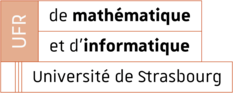
\includegraphics[width=0.40\textwidth]{images/logo_ufr.png}

    \vspace{1.5cm}

    {\large \textcolor{gray}{M1 CSMI - Université de Strasbourg}}

    \vspace{2cm}
    \hrule height 1.5pt
    \vspace{0.8cm}

    {\Huge \textbf{Anomaly Detection on Time-Series Data }}\\[0.5cm]
    {\textcolor{gray}{Application to the MIT-BIH Arrhythmia Database}}
    \vspace{0.8cm}

    \hrule height 1.5pt
    \vspace{2cm}

    {\large Mary Ammar}

    \vspace{0.5cm}
    

    \vspace{1.5cm}
    {\large Supervisor: Christophe Prud'homme}

    \vfill


    {\small \textcolor{gray}{Internship / Defect Detection Project}}


\end{titlepage}




\tableofcontents
\newpage

\section{Introduction}


Every heartbeat produces a small electrical signal that travels through the body and can be
recorded at the skin's surface. The resulting trace from the electrocardiogram (ECG)
is one of the oldest and most widely used diagnostic tools in medicine. In a healthy heart,
this signal repeats itself (same characteristic shape) beat after beat. When something
goes wrong, the shape and timing of the beat change. These irregularities are called 
arrhythmias and some of them are early warnings of serious cardiac conditions.\\

The difficulty is that arrhythmias are rare. Over twenty-four hours of monitoring,
a patient produces more than a hundred thousand beats of which only a small fraction are
abnormal. Reviewing such a recording manually is slow, tiring, precisely because the 
interesting events are buried in a vast amount of unremarkable data. The only solution is 
to automate the search by building a system that learns what a normal beat looks like
and flags anything that departs from it.\\

This problem isn't unique to medicine. In industry, rotating machines produce vibration
signals that behave the same way. A machine in good condition vibrates with a stable
repetitive pattern. As a fault develops, whether through misalignment or a growing crack,
that pattern changes before the machine actually fails. Detecting these early changes 
is the foundation of predictive maintenance which aims to intervene before a breakdown
rather than after it.\\

Despite coming from different worlds, the two situations share the same structure.
In both, we observe a one-dimensional signal that evolves over time, the signal is mostly normal
and occasionally not. In both the central question is the same: how can a system
automatically recognise what departs from normal behavior, without being told in advance
what every possible abnormality looks like?\\

This last point is what makes the problem interesting rather than
routine. Anomalies are not simply a second class to be recognised alongside the first.
They are rare, varied and new ones can always appear. What we need is a methos that 
builds a strong model of normality and treats significaant deviation from it as suspicious. \\

The aim of this internship is to develop, implement and evaluate methods for detecting 
anomalies in the time-series signals, using ECG as the main case study and considering
vibration signals as an extension of the same framework. The work will rely on the MIT-BIH
Arrhythmia database, distributed by PhysioNet. 




\end{document}